%% 
%% Copyright 2007, 2008, 2009 Elsevier Ltd
%% 
%% This file is part of the 'Elsarticle Bundle'.
%% ---------------------------------------------
%% 
%% It may be distributed under the conditions of the LaTeX Project Public
%% License, either version 1.2 of this license or (at your option) any
%% later version.  The latest version of this license is in
%%    http://www.latex-project.org/lppl.txt
%% and version 1.2 or later is part of all distributions of LaTeX
%% version 1999/12/01 or later.
%% 
%% The list of all files belonging to the 'Elsarticle Bundle' is
%% given in the file `manifest.txt'.
%% 

%% Template article for Elsevier's document class `elsarticle'
%% with numbered style bibliographic references
%% SP 2008/03/01

\documentclass[preprint,12pt, a4paper]{elsarticle}

%% Use the option review to obtain double line spacing
%% \documentclass[authoryear,preprint,review,12pt]{elsarticle}

%% For including figures, graphicx.sty has been loaded in
%% elsarticle.cls. If you prefer to use the old commands
%% please give \usepackage{epsfig}

%% The amssymb package provides various useful mathematical symbols
\usepackage{amssymb}
%% The amsthm package provides extended theorem environments
%% \usepackage{amsthm}

%% The lineno packages adds line numbers. Start line numbering with
%% \begin{linenumbers}, end it with \end{linenumbers}. Or switch it on
%% for the whole article with \linenumbers.
\usepackage{lineno}

\usepackage{bm}
\usepackage{tikz}
\usetikzlibrary{positioning,shapes,arrows,calc,intersections}

\journal{SoftwareX}

\begin{document}

\begin{frontmatter}

%% Title, authors and addresses

%% use the tnoteref command within \title for footnotes;
%% use the tnotetext command for theassociated footnote;
%% use the fnref command within \author or \address for footnotes;
%% use the fntext command for theassociated footnote;
%% use the corref command within \author for corresponding author footnotes;
%% use the cortext command for theassociated footnote;
%% use the ead command for the email address,
%% and the form \ead[url] for the home page:
%% \title{Title\tnoteref{label1}}
%% \tnotetext[label1]{}
%% \author{Name\corref{cor1}\fnref{label2}}
%% \ead{email address}
%% \ead[url]{home page}
%% \fntext[label2]{}
%% \cortext[cor1]{}
%% \address{Address\fnref{label3}}
%% \fntext[label3]{}

\title{Splipy}

%% use optional labels to link authors explicitly to addresses:
%% \author[label1,label2]{}
%% \address[label1]{}
%% \address[label2]{}

\author{K.~A.~Johannessen}
\author{E.~Fonn}

\address{SINTEF Digital, PO Box 4760, 7465, Trondheim, Norway}

\begin{abstract}
%% Text of abstract (Ca 100 words)
Splipy is a pure python library for the creation, evaluation and manipulation of B-spline and NURBS geometries.
It supports $n$-variate splines of any dimension, but emphasis is made on the use of curves, surfaces and volumes.
The library is designed primarily for analysis use, and therefore allows fine-grained control over many aspects which is not possible to achieve with conventional CAD tools.

\end{abstract}

\begin{keyword}
%% keywords here, in the form: keyword \sep keyword
NURBS \sep B-splines \sep CAD \sep Interpolation \sep Approximation

%% PACS codes here, in the form: \PACS code \sep code

%% MSC codes here, in the form: \MSC code \sep code
%% or \MSC[2008] code \sep code (2000 is the default)

\end{keyword}

\end{frontmatter}

\linenumbers

%% main text

\section{Motivation and significance}
\label{sec:motivation}

Non-uniform rational B-splines (NURBS) have been a staple technology in \emph{computer aided design} (CAD) for many decades (CITATION NEEDED).
Their mathematical precision allows the user to create smooth parametric descriptions of curves and surfaces, which is necessary in many engineering applications.
Recent years has seen an increased interest in the use of B-splines and NURBS directly in high-fidelity physics simulations such as the finite element method, thereby uniting geometric modelling and analysis.
The groundbreaking work for these methods, termed \emph{isogeometric analysis} (IGA) can be found in \cite{hughes2005iac}.
While commercial CAD tools do well to facilitate NURBS-based modelling, IGA requires finer control of discretization details, and these are often hidden from the user.
We propose Splipy as a modern easy-to-use Python library that will allow scientist and engineers the detailed control that they need to not only make B-spline meshes that are optimized for analysis, but also work well for modelling.

The software allows for rapid generation of high-quality meshes that can be used directly in IGA programs.
While Splipy offers everything needed in terms of basis function evaluations, derivatives etc.~to build a stand-alone finite element solver, we envision that most users will be content to generate the geometry in Splipy followed by exporting to external solvers.

% \begin{itemize}
%   \item Introduce the scientific background and the motivation for developing the software.
%   \item Explain why the software is important, and describe the exact (scientific) problem(s) it solves.
%   \item Indicate in what way the software has contributed (or how it will contribute in the future) to the process of scientific discovery; if available, this is to be supported by citing a research paper using the software.
%   \item Provide a description of the experimental setting (how does the user use the software?).
%   \item Introduce related work in literature (cite or list algorithms used, other software etc.).
% \end{itemize}

\section{Software description}
\label{sec:description}

The core tenet of Splipy is the manipulation of \emph{spline objects}, by which is meant a mapping from a $n$-dimensional \emph{parameter space},
\begin{equation}
  \label{eqn:paramspace}
  \mathcal{P} = [l_1, r_1] \times [l_2, r_2] \times \cdots \times [l_n, r_n]
\end{equation}
into \emph{physical space} $\mathbb{R}^d$.
Conventionally, $d \geq n$.
In spline terms, each parameter interval $[l_i, r_i]$ is subdivided into a \emph{knot vector}
\begin{equation}
  \label{eqn:knotvector}
  l_i = k_0 \leq k_1 \leq k_2 \leq \cdots \leq k_{n_i} = r_i,
\end{equation}
with nondecreasing \emph{knots} $k_j$.
Given a knot vector and a polynomial degree $p_i$, there is a unique B-spline basis $B_j(x_i)$ defined on the interval $[l_i, r_i]$.
Each basis function $B_j$ is piecewise polynomial with degree $p_i$ in all knot intervals $[k_m, k_{m+1}]$, and is supported on exactly $p_i+1$ such intervals.

Given a choice of knot vector and degree for each direction $i=1,\ldots,n$, the full B-spline basis is defined on $\mathcal{P}$ as
\begin{equation}
  \label{eqn:bspline-multi}
  B_{j_1,\ldots,j_n}(x_1,\ldots,x_n) = B_{j_1}(x_1) \cdots B_{j_n}(x_n)
\end{equation}
and a \emph{spline object} is nothing more than a function in the span of this basis, i.e.~a function $s: \mathcal{P} \to \mathbb{R}^d$ such that
\begin{equation}
  \label{eqn:splineobj}
  s(\bm x) = \sum_{j_1, \ldots, j_n} \bm c_{j_1, \ldots, j_n} B_{j_1, \ldots, j_n}(\bm x).
\end{equation}
Here, the coefficients $\bm c_{j_1, \ldots, j_n} \in \mathbb{R}^d$ are termed \emph{control points}.

Splipy is concerned with the creation and manipulation of these mappings and the objects they represent (that is, the image of $\mathcal{P}$ by $s$ in $\mathbb{R^d}$).
Since the objective is analysis, and since the smoothness properties of the basis functions depend crucially on the knot vector, and since the element sizes and shapes depend crucially on the control points, fine control over these quantities are important.

\subsection{Software Architecture}
\label{sec:architecture}

There are three main classes which are exposed to the user: \texttt{Curve}, \texttt{Surface} and \texttt{Volume}.
All inherit from the \texttt{SplineObject} superclass, which contains common methods such as affine transformations, evaluation and get methods.
See Figure~\ref{fig:hierarchy}.
It is possible to create such spline objects manually, by specifying knot vectors and control points, however most users will be using a wide range of ``factory'' functions for creating simple geometries.
These can be found in the submodules \texttt{curve\_factory}, \texttt{surface\_factory} and \texttt{volume\_factory}.
More advanced geometries can then be created by using the rich interface for manipulating spline objects.
Generally Splipy scripts follow a bottom-up construction scheme where curves are created from points, surfaces are created from curves and finally volumes are created from the surfaces.

\begin{figure}
  \begin{center}
    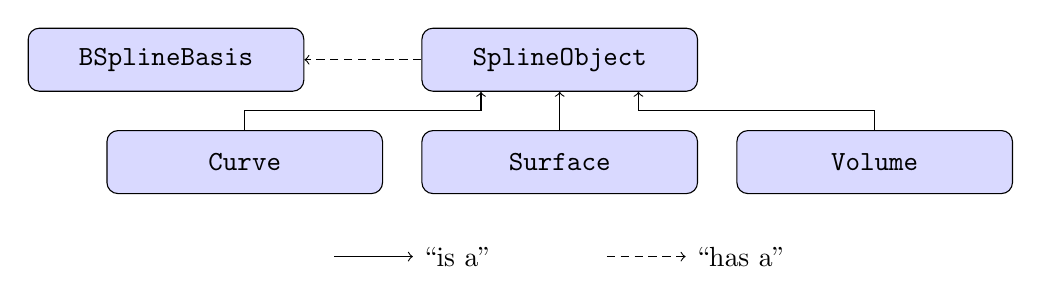
\begin{tikzpicture}[
      class/.style={rectangle, draw=black, fill=blue!15, align=center, rounded corners, minimum width=3.5cm, minimum height=0.8cm},
      ]
      \node[class] (BS) at (-5.0,0) {\texttt{BSplineBasis}};
      \node[class] (SO) at (0,0) {\texttt{SplineObject}};
      \node[class] (CU) at (-4.0,-1.3) {\texttt{Curve}};
      \node[class] (SF) at (0,-1.3) {\texttt{Surface}};
      \node[class] (VO) at (4.0,-1.3) {\texttt{Volume}};

      \draw[->] (SF.north) -- (SO.south);
      \draw[->] (CU.north) -- ++(0,0.25) -| ([xshift=-1cm]SO.south);
      \draw[->] (VO.north) -- ++(0,0.25) -| ([xshift=1cm]SO.south);
      \draw[->, densely dashed] (SO.west) -- (BS.east);

      \node (isa) at (-1.3,-2.5) {``is a''};
      \draw[->] ([xshift=-1cm]isa.west) -- (isa.west);

      \node (hasa) at (2.3,-2.5) {``has a''};
      \draw[->, densely dashed] ([xshift=-1cm]hasa.west) -- (hasa.west);
    \end{tikzpicture}
  \end{center}
  \label{fig:hierarchy}
  \caption{Class hierarchy of Splipy.}
\end{figure}

\subsection{Software Functionalities}
\label{}

In addition to elementary objects such as line, circle, disc, sphere, torus, cylinder and teapots, the factory classes contain spline-related constructors such as interpolation, least-square fit and lofting.
Of the more complex methods we draw special attention to \texttt{curve\_factory.fit(...)}.

\subsubsection{Curve fitting}
\label{}

\subsubsection{Interior from edges}
\label{}

Present the major functionalities of the software.

NACA wing profile is created in accordance with \cite{abbott1959tow}

A cubical topology to the volumetric sphere  \cite{cobb1988tts}

\subsection{Sample code snippets analysis (optional)}
\label{}

\section{Illustrative Examples}
\label{}

Provide at least one illustrative example to demonstrate the major functions.

Optional: you may include one explanatory video that will appear next to your article, in the right hand side panel. (Please upload any video as a single supplementary file with your article. Only one MP4 formatted, with 50MB maximum size, video is possible per article. Recommended video dimensions are 640 x 480 at a maximum of 30 frames/second. Prior to submission please test and validate your .mp4 file at $ http://elsevier-apps.sciverse.com/GadgetVideoPodcastPlayerWeb/verification$. This tool will display your video exactly in the same way as it will appear on ScienceDirect.).

\section{Impact}
\label{}

\textbf{This is the main section of the article and the reviewers weight the description here appropriately}

Indicate in what way new research questions can be pursued as a result of the software (if any).

Indicate in what way, and to what extent, the pursuit of existing research questions is improved (if so).

Indicate in what way the software has changed the daily practice of its users (if so).

Indicate how widespread the use of the software is within and outside the intended user group.

Indicate in what way the software is used in commercial settings and/or how it led to the creation of spin-off companies (if so).

\section{Conclusions}
\label{}

Set out the conclusion of this original software publication.

\section*{Acknowledgements}
\label{}

Optionally thank people and institutes you need to acknowledge. 

%% The Appendices part is started with the command \appendix;
%% appendix sections are then done as normal sections
%% \appendix

%% \section{}
%% \label{}

%% References:
%% If you have bibdatabase file and want bibtex to generate the
%% bibitems, please use
%%
\bibliographystyle{elsarticle-num}{}
\bibliography{references}

%% else use the following coding to input the bibitems directly in the
%% TeX file.

%% \begin{thebibliography}{00}

%% \bibitem{label}
%% Text of bibliographic item

%% \bibitem{}

%% \end{thebibliography}

\section*{Required Metadata}
\label{}

\section*{Current code version}
\label{}

Ancillary data table required for subversion of the codebase. Kindly replace examples in right column with the correct information about your current code, and leave the left column as it is.

\begin{table}[!h]
\begin{tabular}{|l|p{6.5cm}|p{6.5cm}|}
\hline
\textbf{Nr.} & \textbf{Code metadata description} & \textbf{Please fill in this column} \\
\hline
C1 & Current code version & 1.3 \\
\hline
C2 & Permanent link to code/repository used for this code version & $https://github.com/sintefmath/splipy$ \\
\hline
C3 & Legal Code License   & GNU General Public License v3.0  \\
\hline
C4 & Code versioning system used & git \\
\hline
C5 & Software code languages, tools, and services used & python \\
\hline
C6 & Compilation requirements, operating environments \& numpy $\geq$ 1.9, scipy $\geq$ 0.17 \\
\hline
C7 & If available Link to developer documentation/manual & $https://sintefmath.github.io/Splipy/$ \\
\hline
C8 & Support email for questions & Kjetil.Johannessen@sintef.no \\
\hline
\end{tabular}
\caption{Code metadata (mandatory)}
\label{} 
\end{table}

\section*{Current executable software version}
\label{}

Ancillary data table required for sub version of the executable software: (x.1, x.2 etc.) kindly replace examples in right column with the correct information about your executables, and leave the left column as it is.

\begin{table}[!h]
\begin{tabular}{|l|p{6.5cm}|p{6.5cm}|}
\hline
\textbf{Nr.} & \textbf{(Executable) software metadata description} & \textbf{Please fill in this column} \\
\hline
S1 & Current software version & 1.3 \\
\hline
S2 & Permanent link to executables of this version  & $https://github.com/sintefmath/splipy$ \\
\hline
S3 & Legal Software License & GNU General Public License v3.0 \\
\hline
S4 & Computing platforms/Operating Systems & Linux, OS X, Microsoft Windows, Unix-like \\
\hline
S5 & Installation requirements \& dependencies & numpy $\geq$ 1.9, scipy $\geq$ 0.17 \\
\hline
S6 & If available, link to user manual - if formally published include a reference to the publication in the reference list & $https://sintefmath.github.io/Splipy/$ \\
\hline
S7 & Support email for questions & Kjetil.Johannessen@sintef.no \\
\hline
\end{tabular}
\caption{Software metadata (optional)}
\label{} 
\end{table}

\end{document}
\endinput
%%
%% End of file `SoftwareX_article_template.tex'.
